\documentclass[a4paper,10pt]{jsarticle}
\usepackage{amsmath,amssymb}
\usepackage{bm}
\usepackage[subrefformat=parens]{subcaption}
\usepackage[dvipdfmx]{graphicx}
\usepackage[dvipdfmx]{color}

\title{Machine Learning Midterm Assignment}
\author{Keisuke Okumura, 18M31013}

\newcommand{\argmax}{\mathop{\rm argmax}\limits}
\newcommand{\argmin}{\mathop{\rm argmin}\limits}
\newcommand{\coloneq}{:=}

\begin{document}
\maketitle

\section*{Problem 1}
ロジスティック回帰では次の問題を解くことになる.
\[ \hat{\bm{w}} = \argmin_{\bm{w}}J(\bm{w}) \]
\[
 J(\bm{w}) \coloneq \sum_{i=1}^{n}(
 \ln{(1 + \exp{(-y_i\bm{w}^\mathrm{T}\bm{x}_i)}}))
 + \lambda \bm{w}^\mathrm{T}\bm{w}
\]

最急降下法(steepest gradient method)では, 以下の更新式に従って学習を行う. $\alpha$ は定数とする.
\[
\bm{w}^{(t+1)} = \bm{w}^{(t)} - \alpha\left.\frac{\partial J}{\partial \bm{w}}\right|_{\bm{w}=\bm{w}^{(t)}}
\]
\begin{align*}
\frac{\partial J(\bm{w})}{\partial \bm{w}}
 &= \frac{1}{n}\sum_{i=1}^{n}
 \frac{\exp(-y_i\bm{w}^\mathrm{T}\bm{x}_i)(-y_i\bm{x}_i)}
 {1 + \exp(-y_i\bm{w}^\mathrm{T}\bm{x}_i)}
 + 2\lambda\bm{w}\\
 &=\frac{1}{n}\sum_{i=1}^{n}
 \frac{-y_i\bm{x}_i}
 {1 + \exp(y_i\bm{w}^\mathrm{T}\bm{x}_i)}
 + 2\lambda\bm{w}\\
\end{align*}

また, ニュートン法(newton method)では以下の更新式に従って学習を行う. $\alpha$ は定数とする.
\[ \bm{w}^{(t+1)} = \bm{w}^{(t)} + \alpha\bm{d}^{(t)} \]
\[ \nabla^2J(\bm{w}^{(t)})\bm{d}^{(t)} = -\nabla J(\bm{w}^{(t)})
\Longleftrightarrow
\bm{d}^{(t)} = - (\nabla^2J(\bm{w}^{(t)}))^{-1} \nabla J(\bm{w}^{(t)})
\]

$\nabla^2J(\bm{w})$は次のように計算される.
\[
 \nabla^2J(\bm{w}) = \frac{1}{n}\sum_{i=1}^{n}
 \left(\frac{\exp(-y_i\bm{w}^\mathrm{T}\bm{x}_i)}
 {(1 + \exp(-y_i\bm{w}^\mathrm{T}\bm{x}_i))^2}\bm{x}_i\bm{x}_i^\mathrm{T}\right) + 2\lambda\bm{I}
\]

$100$個のデータからなるデータセットを Toy Dataset I\hspace{-1pt}I を参考に生成し,
最急降下法, 及びニュートン法を実行した結果を図.~\ref{img:log-result}に示す.
また, その時の学習の進行の様子を図.~\ref{img:log-loss}に示す.
パラメータ更新の繰り返し数は$50$回, $\alpha=0.1$, $\lambda=0.1$として学習を行った.

\begin{figure}[htbp]
 \begin{minipage}{0.5\hsize}
  \begin{center}
   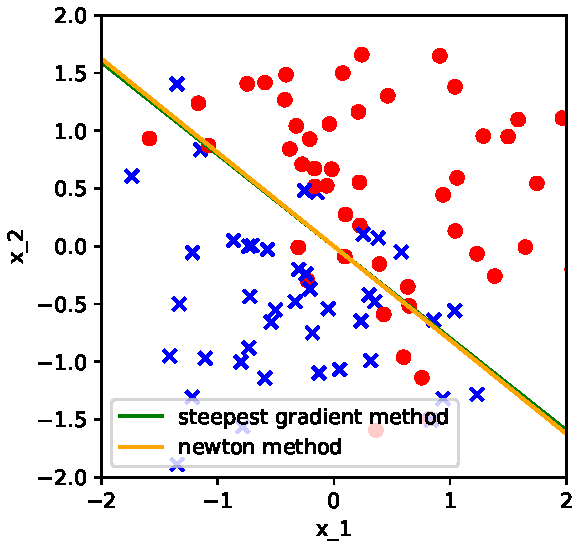
\includegraphics[width=7cm]{figs/p1_logistic-regression_result.pdf}
  \end{center}
  \caption{ロジスティック回帰の学習結果. $\bm{w}^\mathrm{T}\bm{x}=0$ を描画.}
  \label{img:log-result}
 \end{minipage}
 \begin{minipage}{0.5\hsize}
  \begin{center}
   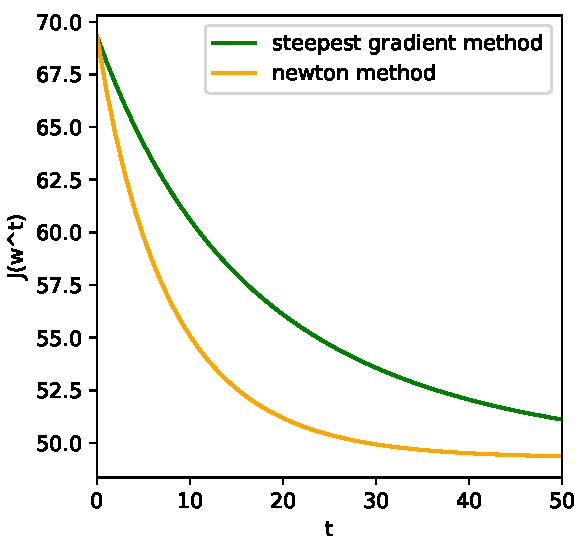
\includegraphics[width=7cm]{figs/p1_logistic-regression_loss.pdf}
  \end{center}
  \caption{損失関数の値の変化.}
  \label{img:log-loss}
 \end{minipage}
\end{figure}

\section*{Problem 2}
本問題では, \textit{lasso}を用いて次の問題を考える.
\[
 \hat{\bm{w}} = \argmin_{\bm{w}}((\bm{w}-\bm{\mu})^\mathrm{T}\bm{A}(\bm{w}-\bm{\mu})
 + \lambda||\bm{w}||_1)
\]
解を得るために, Proximal gradient method (PG) を用いる.
$\psi = (\bm{w}-\bm{\mu})^\mathrm{T}\bm{A}(\bm{w}-\bm{\mu})$ とする.
更新式は次のようになる.
\begin{align*}
 w^{(t+1)}_i
 &= prox_{\eta_t\lambda||\cdot||_1}\left(\bm{w}^{(t)}
 - \eta_t\nabla\psi(\bm{w}^{(t)})\right)
\end{align*}
ここで, 学習率 $\eta_t=\gamma^{-1}$ とする.
$\gamma$ は $\psi$ のリプシッツ定数とし, $2\bm{A}$ の固有値の最大値をとることができる.
上式はL1ノルムの近接写像であるから, Soft Threshold関数を用いて, 次のように変換される.
\begin{align*}
 w^{(t+1)}_i
 = ST_{\frac{\lambda}{\gamma}}\left(w^{(t)}_i
 -\left\{\frac{1}{\gamma}\nabla\psi(\bm{w}^{(t)})\right\}_i\right),
 \,\,\,\,
 ST_q(\mu) = \begin{cases}
              \mu - q &(\mathit{if} \,\, \mu > q)\\
              0 &(\mathit{if} \,\, |\mu| \leq q)\\
              \mu + q &(\mathit{if} \,\, \mu < -q)\\
             \end{cases}
\end{align*}

$\psi$ を二次形式とみなし $\bm{A}$ を対称行列とすると, $\nabla \psi$ は次のようになる.
\[
 \nabla \psi = (\bm{A} + \bm{A}^\mathrm{T})(\bm{w} - \bm{\mu}) = 2\bm{A}(\bm{w} - \bm{\mu})
\]

以上より, 更新式は次式で表される.
\[
 w^{(t+1)}_i
 = ST_{\frac{\lambda}{\gamma}}\left(w^{(t)}_i
 -\left\{\frac{1}{\gamma}2\bm{A}(\bm{w}^{(t)} - \bm{\mu})\right\}_i\right)
\]

また, Accelerated proximal gradient (APG) を用いた場合, 更新式は次のように変化する.
\[
  \bm{w}^{(t+1)} = prox_{\eta_t\lambda||\cdot||_1}\left(
 \bm{v}^{(t)} - \eta_t\nabla\psi(\bm{v}^{(t)})\right)
\]
\[ \bm{v}^{(t)} = \bm{w}^{(t)} + q(t)(\bm{w}^{(t)} - \bm{w}^{(t-1)}) \]
$q(t)$はスカラー関数である. 今回は次式を用いる.
\[ q(t) = \frac{t-1}{t+2} \]

以上を踏まえて, 以下の条件で学習を行う.
\[
 \bm{A} = \left(\begin{array}{cc} 3 & 0.5 \\ 0.5 & 1 \end{array}\right), \,
 \bm{\mu} = \left(\begin{array}{c} 1 \\ 2 \end{array}\right)
\]

繰り返し数を$50$回, $\lambda$ を$2$, $4$, $6$と変えた時の学習の様子を図.~\ref{img:lasso-result}に示す.
さらに, Python の数理最適化ライブラリ CVXOPT を使用して最適解 $\hat{\bm{w}}$ を導出し,
$||\bm{w}^{(t)} - \hat{\bm{w}}||_1$ を計算して結果を図.~\ref{img:lasso-error}に示す.

\begin{figure}[htbp]
 \begin{minipage}{0.33\hsize}
  \begin{center}
   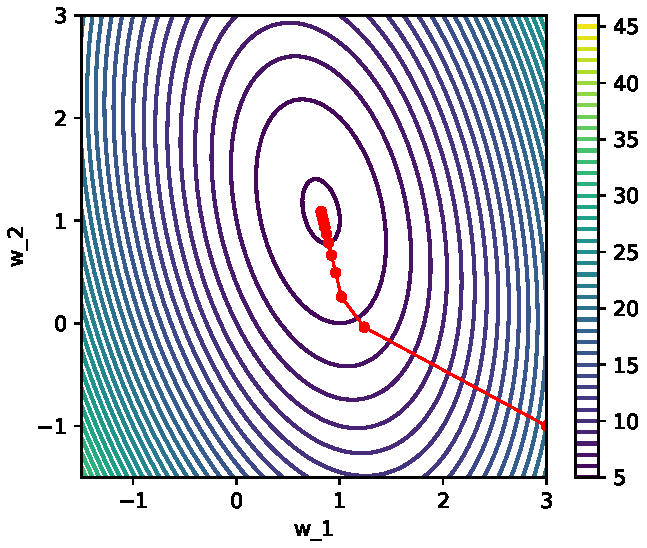
\includegraphics[width=5cm]{figs/p2_lasso_result_lambda-2.pdf}
  \end{center}
 \end{minipage}
 \begin{minipage}{0.33\hsize}
  \begin{center}
   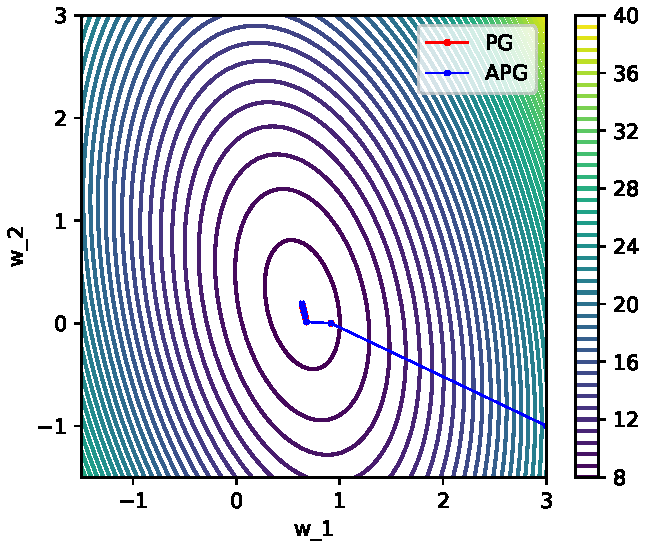
\includegraphics[width=5cm]{figs/p2_lasso_result_lambda-4.pdf}
  \end{center}
 \end{minipage}
 \begin{minipage}{0.33\hsize}
  \begin{center}
   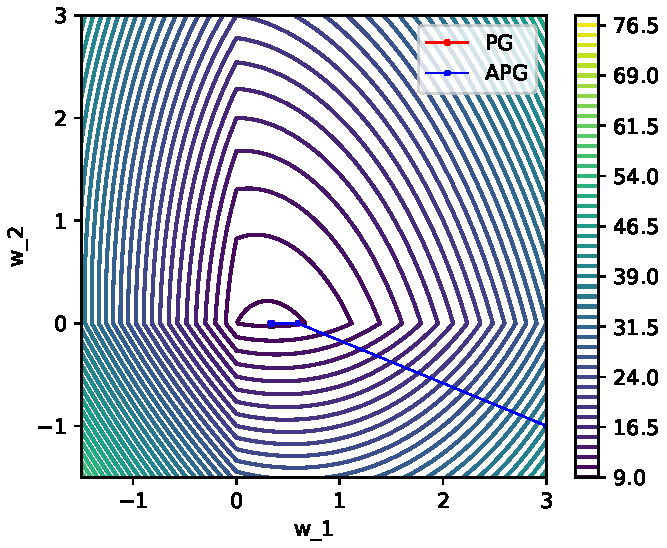
\includegraphics[width=5cm]{figs/p2_lasso_result_lambda-6.pdf}
  \end{center}
 \end{minipage}
 \caption{\textit{lasso} を用いて学習を行った様子. 
 左から $\lambda=2, 4, 6$となっている.}
 \label{img:lasso-result}
\end{figure}

\begin{figure}[htbp]
 \begin{minipage}{0.33\hsize}
  \begin{center}
   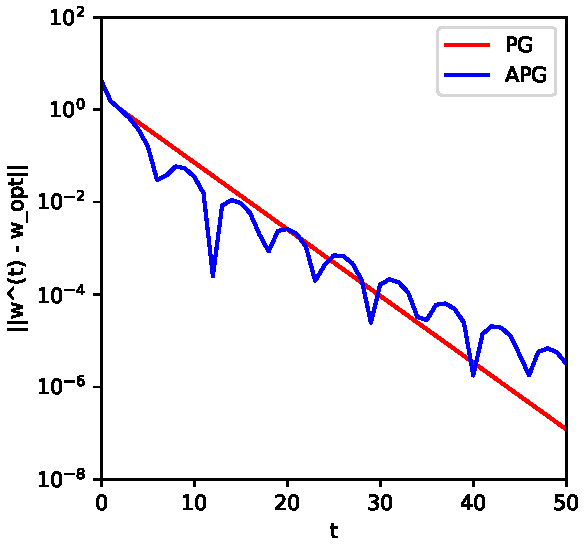
\includegraphics[width=5cm]{figs/p2_lasso_dist_lambda-2.pdf}
  \end{center}
 \end{minipage}
 \begin{minipage}{0.33\hsize}
  \begin{center}
   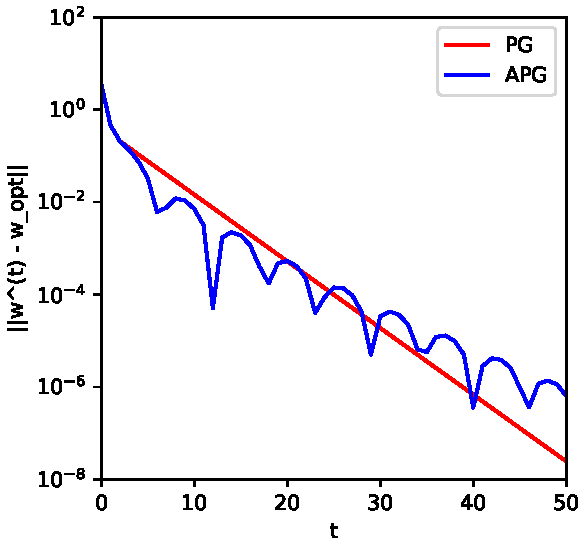
\includegraphics[width=5cm]{figs/p2_lasso_dist_lambda-4.pdf}
  \end{center}
 \end{minipage}
 \begin{minipage}{0.33\hsize}
  \begin{center}
   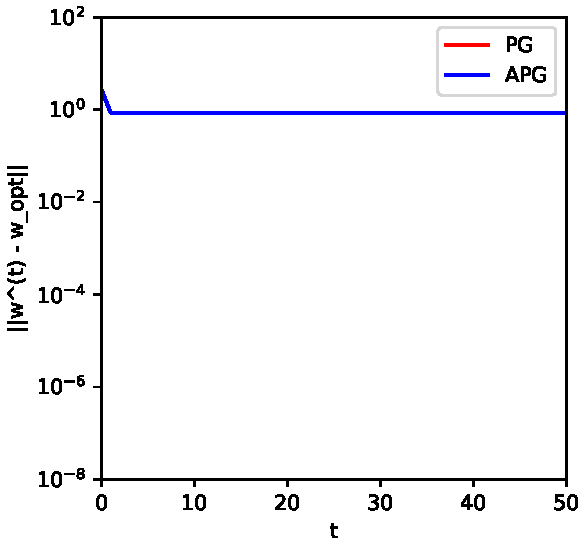
\includegraphics[width=5cm]{figs/p2_lasso_dist_lambda-6.pdf}
  \end{center}
 \end{minipage}
 \caption{\textit{lasso}を用いて学習した時の$||\bm{w}^{(t)} - \hat{\bm{w}}||_1$の値の変化.
 左から $\lambda=2, 4, 6$となっている.
 $\lambda=6$の時, PG と APG の線はほとんどかぶっている.}
 \label{img:lasso-error}
\end{figure}

AdaGrad を使用した場合, \textit{lasso}の更新式は次のようになる.
\[
  \bm{w}^{(t)}
 = \argmin_{\bm{w}}\left((\bm{w} - \bm{w}^{(t-1)})^\mathrm{T}\bm{g}_t+\lambda||\bm{w}||_1
 +\frac{1}{2\eta_0}||\bm{w}-\bm{w}^{(t-1)}||^2_{\bm{H}_t}\right)
\]
ただし, $\bm{g}_t=\nabla\psi(\bm{w}^{(t-1)})$ である.
$\bm{H}_t$ は次のように定義される.
\[
 \bm{H}_t = \bm{G}^{1/2}_t + \epsilon\bm{I},\,\,\,\,
  \{\bm{G_t}\}_{i,j}=\delta_{ij}\sum_{\tau=1}^{t}\{\bm{g}_{\gamma}\}^2_i
\]
更新式はSoft Threshold関数を用いると, 次のように表される.
\[
 \bm{w}^{(t)}_i = ST_{\eta_0\lambda\{\bm{H}_t^{-1}\}_{ii}}
 \left(\bm{w}^{(t-1)}_i-\eta_0\{\bm{H}^{-1}_t\bm{g}_t\}_i\right)\\
\]

PG, APG, AdaGrad の比較を行う. 以下の条件で学習を行う.
\[
 \bm{A} = \left(\begin{array}{cc} 250 & 15 \\ 15 & 4 \end{array}\right), \,
 \bm{\mu} = \left(\begin{array}{c} 1 \\ 2 \end{array}\right), \,
 \lambda = 0.89
\]
AdaGrad のパラメータとして, $\eta_0=500/\gamma$, $\epsilon=0.02$を用いた.

繰り返し数を$500$回とした時の学習の様子と,
CVXOPT により導出された最適解$\hat{\bm{w}}$を用いて
$||\bm{w}^{(t)} - \hat{\bm{w}}||_1$を計算し,
その結果を図.~\ref{img:lasso-adagrad}に示す.
\begin{figure}[htbp]
 \begin{minipage}{0.5\hsize}
  \begin{center}
   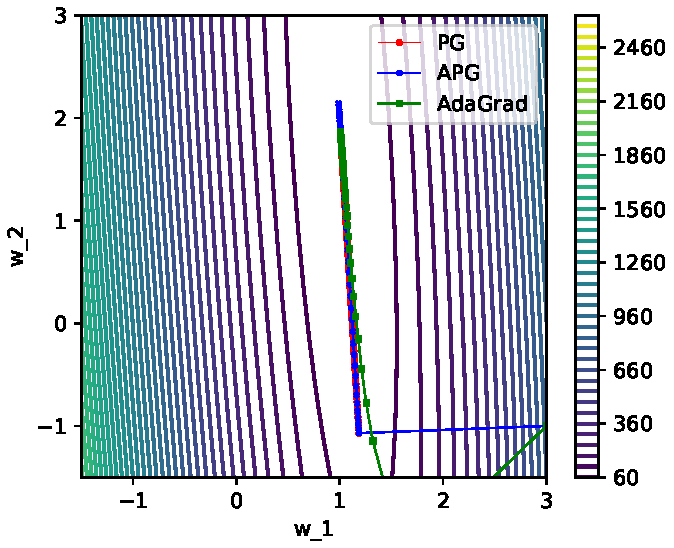
\includegraphics[width=7cm]{figs/p2_lasso_result_pg-apg-adagrad.pdf}
  \end{center}
  \vspace{-0.5cm}
  \subcaption{}
 \end{minipage}
 \begin{minipage}{0.5\hsize}
  \begin{center}
   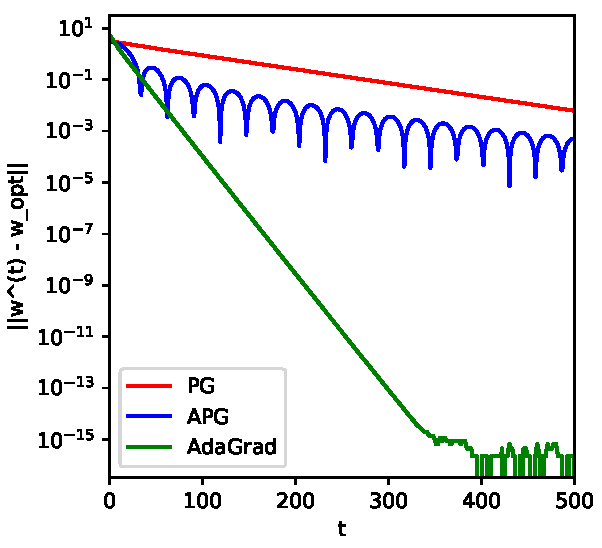
\includegraphics[width=7cm]{figs/p2_lasso_dist_adagrad.pdf}
  \end{center}
  \vspace{-0.5cm}
  \subcaption{}
 \end{minipage}
 \caption{\textbf{a)} \textit{lasso} を用いて学習を行った様子.
 \textbf{b)} $||\bm{w}^{(t)} - \hat{\bm{w}}||_1$の値の変化.
 }
 \label{img:lasso-adagrad}
\end{figure}

\section*{Problem 3}
support vector machine では次の問題を考える. $\lambda > 0$とする.
\begin{equation}
 \hat{\bm{w}} = \argmin_{w \in \mathbb{R}^d}
  \left(\sum_{i=1}^{n}max(0, 1 - y_i\bm{w}^\mathrm{T}\bm{x}_i)
   + \lambda||\bm{w}||^2_2 \right)
\end{equation}
$\xi_i \geq max(0, 1 - y_i\bm{w}\mathrm{T}\bm{x}_i) \geq 0$ となる
$\bm{\xi} = (\xi_1, ..., \xi_n)^\mathrm{T}$を用いて,
上記の問題を以下の最適化問題に置き換える.
$C=1/2\lambda$とする.
\begin{align*}
 minimize_{\bm{w}, \bm{\xi}} \,\,\,\,
 & \frac{1}{2}\bm{w}^\mathrm{T}\bm{w} + C\bm{1}^\mathrm{T}\bm{\xi}\\
 subject \,\, to \,\,\,\, &\xi_i \geq 1 - y_i\bm{w}^\mathrm{T}\bm{x}_i\\
 &\xi_i \geq 0
\end{align*}
Lagrangian を求めると以下のようになる.
\begin{align*}
 L(\bm{w}, \bm{\xi}, \bm{\alpha}, \bm{\beta})
 = \frac{1}{2}\bm{w}^\mathrm{T}\bm{w} + C\bm{1}^\mathrm{T}\bm{\xi}
 + \sum_{i}\alpha_i(1 - y_i\bm{w}^\mathrm{T}\bm{x}_i - \xi_i)
 + \sum_{i}\beta_i(-\xi_i)
\end{align*}
KKT 条件を求める.
\begin{align*}
 \frac{\partial L}{\partial \bm{w}} = 0 \,\, \Longleftrightarrow
 &\,\,\hat{\bm{w}} = \sum_{i}\alpha_iy_i\bm{x}_i\\
 \frac{\partial L}{\partial \bm{\xi}} = 0 \,\, \Longleftrightarrow
 &\,\,\hat{\bm{\alpha}} + \hat{\bm{\beta}} = C\bm{1}\\
 \hat{\alpha}_i \geq 0\\
 \hat{\beta}_i \geq 0\\
 \hat{\alpha}_i(1 - y_i\hat{\bm{w}}^\mathrm{T}\bm{x}_i - \hat{\xi}_i) = 0\\
 \hat{\beta}_i(- \hat{\xi}_i) = 0
\end{align*}
次に, Lagrange の双対関数を求める.
$\hat{\bm{w}}=\sum_{i}\alpha_iy_i\bm{x}_i$,
$\hat{\bm{\beta}} = C\bm{1} - \hat{\bm{\alpha}}$
を利用する.
\begin{align*}
 \tilde{L}(\bm{\alpha}, \bm{\beta})
 & = \inf_{\bm{w}, \bm{\xi} \in D}L(\bm{w}, \bm{\xi}, \bm{\alpha}, \bm{\beta})\\
 & = \frac{1}{2}\left(\sum_{i}\alpha_iy_i\bm{x}_i\right)^\mathrm{T}
 \left(\sum_{i}\alpha_iy_i\bm{x}_i\right)
 + C\bm{1}^\mathrm{T}\bm{\xi}\\
 &\,\,\,\,\,\,\,\,+ \sum_{i}\alpha_i\left(1 - y_i
 \left(\sum_{j}\alpha_jy_j\bm{x}_j\right)^\mathrm{T}\bm{x}_i-\xi_i\right)\\
 &\,\,\,\,\,\,\,\,+ \sum_i(C - \alpha_i)(-\xi_i)\\
 & = \sum_i\alpha_i - \frac{1}{2}\sum_{i,j}\alpha_i\alpha_jy_iy_j
 \bm{x}^\mathrm{T}_i\bm{x}_j\\
 & = -\frac{1}{2}\bm{\alpha}^\mathrm{T}\bm{K}\mathrm{\bm{\alpha}}
 + \bm{\alpha}^\mathrm{T}\bm{1}
\end{align*}
したがって双対問題は次のように表される.
\begin{align*}
 maximize_{\bm{\alpha}} \,\,\,\,
 & -\frac{1}{2}\bm{\alpha}^\mathrm{T}\bm{K}\mathrm{\bm{\alpha}}
 + \bm{\alpha}^\mathrm{T}\bm{1}\\
 subject \,\, to \,\,\,\, &\bm{0} \leq \bm{\alpha} \leq C\bm{1}
 = \frac{1}{2\lambda}\bm{1}
\end{align*}
ただし, $\{\bm{K}\}_{i, j} = y_iy_j\bm{x}_i^\mathrm{T}\bm{x}_j$ とする.
ここで $\bm{\alpha} \rightarrow \bm{\alpha}/2\lambda$ とすると,
上記の双対問題を以下のように変形することができ, これが解くべき問題である.
\begin{align}
 maximize_{\bm{\alpha}} \,\,\,\,
 & -\frac{1}{4\lambda}\bm{\alpha}^\mathrm{T}\bm{K}\mathrm{\bm{\alpha}}
 + \bm{\alpha}^\mathrm{T}\bm{1}\\
 subject \,\, to \,\,\,\, &\bm{0} \leq \bm{\alpha} \leq \bm{1}
\end{align}

また, 導出の過程で出てきた $\hat{\bm{w}}$ にも
$\bm{\alpha} \rightarrow \bm{\alpha}/2\lambda$ を適用すると,
最適解は次のように書き下すことができる.
\[ \hat{\bm{w}} = \frac{1}{2\lambda}\sum_{i}\alpha_iy_i\bm{x}_i \]

続いて, projected gradient method を用いて(2)式の解を求める.
$\psi(\bm{\alpha}) = \frac{1}{4\lambda}\bm{\alpha}^\mathrm{T}\bm{K}\mathrm{\bm{\alpha}}
 - \bm{\alpha}^\mathrm{T}\bm{1}$
とすると, ラグランジュの双対問題は$\psi(\bm{\alpha})$の最小化問題とみなすことができる.

projected gradientの更新式は以下の通り.
\begin{align*}
 \bm{\alpha}^{(t)}
 & = P_{[0,1]^n}(\bm{\alpha}^{(t-1)} - \eta_t\nabla\psi(\bm{\alpha}^{(t-1)}))\\
 & = P_{[0,1]^n}\left(\bm{\alpha}^{(t-1)} - \eta_t\left(
 \frac{1}{2\lambda}\bm{K}\bm{\alpha} - \bm{1}\right)\right)
\end{align*}
$P_{[0,1]^n}$は $[0, 1]$ への射影演算子であり, 具体的には次のような写像である.
\[
  \{P_{[0,1]^n}(\tilde{\bm{\alpha}})\}_i
  = \begin{cases}
     0 &(\mathit{if} \,\, \tilde{\alpha}_i < 0)\\
     \tilde{\alpha}_i &(\mathit{if} \,\, 0 \leq \tilde{\alpha}_i \leq 1)\\
     1 &(\mathit{if} \,\, 1 < \tilde{\alpha}_i)
    \end{cases}
\]

以上を踏まえて学習を行う.
繰り返し数を$50$回, $\lambda=10$, $\eta_t = 0.1$ とした時の学習の様子を図~\ref{img:svm}に示す.
\begin{figure}[htbp]
 \begin{minipage}{0.5\hsize}
  \begin{center}
   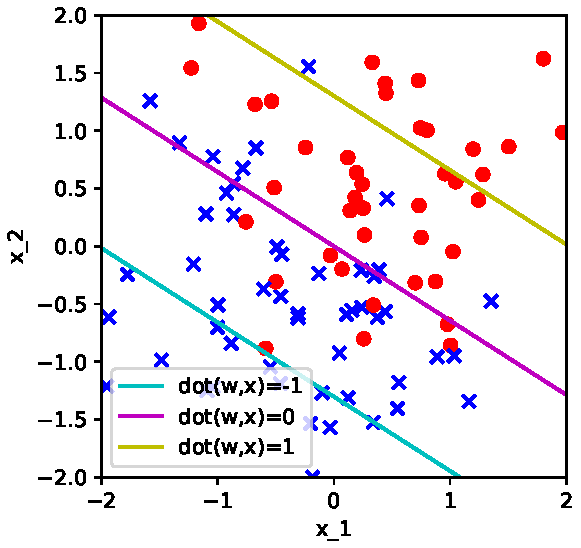
\includegraphics[width=7cm]{figs/p3_svm_result.pdf}
  \end{center}
  \vspace{-0.5cm}
  \subcaption{}
 \end{minipage}
 \begin{minipage}{0.5\hsize}
  \begin{center}
   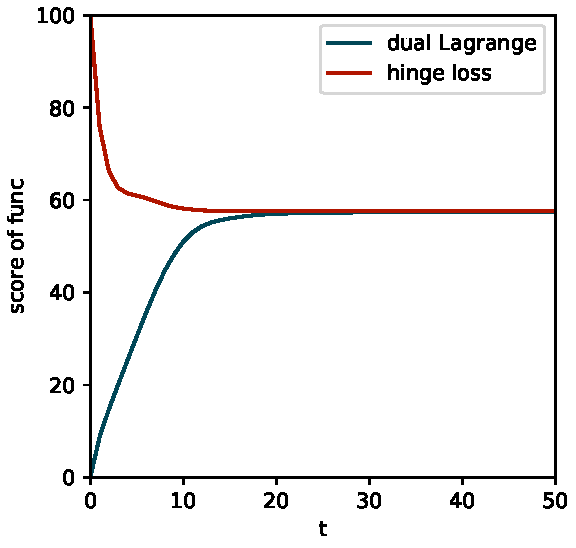
\includegraphics[width=7cm]{figs/p3_svm_gap.pdf}
  \end{center}
  \vspace{-0.5cm}
  \subcaption{}
 \end{minipage}
 \caption{\textbf{a)} \textit{support vector machine} を用いて学習を行った様子.
 $\bm{w}^\mathrm{T}\bm{x}=-1,0,1$を描画.
 \textbf{b)} ヒンジ損失関数と正則化項の和 - (1)式と,
 ラグランジュの双対関数 - (2)式の値の変化の様子.
 duality gapが0に収束していく様子が見られる.}
 \label{img:svm}
\end{figure}

\section*{Problem 4}
ヒンジ損失関数とL1正則化項を用いて, binary classificationの問題を考える.
具体的には次の問題を考える.
\begin{equation}
 \hat{\bm{w}} = \argmin_{w \in \mathbb{R}^d}
  \left(\sum_{i=1}^{n}max(0, 1 - y_i\bm{w}^\mathrm{T}\bm{x}_i)
   + \lambda||\bm{w}||_1 \right)
\end{equation}
$0 \leq \max(0, 1 - y_i\bm{w}\mathrm{T}\bm{x}_i) \leq \xi_i$ となる
$\bm{\xi} = (\xi_1, ..., \xi_n)^\mathrm{T}$と,
$e_i \geq |w_i| \geq 0$ となる
$\bm{e} = (e_1, ..., e_n)^\mathrm{T}$を用いて,
上記の問題を以下の最適化問題に置き換える.
\begin{align*}
 minimize_{\bm{w}, \bm{x}} \,\,\,\,
 & \bm{1}^\mathrm{T}\bm{\xi} + \lambda\bm{1}^\mathrm{T}\bm{e}\\
 subject \,\, to \,\,\,\, &\xi_i \geq 1 - y_i\bm{w}^\mathrm{T}\bm{x}_i\\
 & \xi_i \geq 0\\
 & e_i \geq - w_i\\
 & e_i \geq w_i\\
 & e_i \geq 0
\end{align*}
ここで, $\bm{z}$, $\bm{c}$, $\bm{A}$, $\bm{b}$ を以下のように定義する.
\begin{equation*}
 \bm{z} = \left(\begin{array}{c} \bm{\xi} \\ \bm{e} \\ \bm{w} \end{array}\right), \,\,\,\,
 \bm{c} = \left(\begin{array}{c} \bm{1}^d \\ \lambda\bm{1}^d \\ \bm{0}^d\end{array}\right)\\
\end{equation*}
\begin{equation*}
 \bm{A} = \left(\begin{array}{ccccccccc}
           -1 & & 0 & 0 & \cdots & 0 & -y_1x_{11} & \cdots & -y_1x_{1d} \\
            & \ddots &  & \vdots & & \vdots & \vdots &  & \vdots \\
           0 & & -1 & 0 & \cdots & 0 & -y_1x_{d1} & \cdots & -y_1x_{dd}\\
           -1 & & 0 & 0 & \cdots & 0 & 0 & \cdots & 0 \\
            & \ddots & & \vdots & & \vdots & \vdots & & \vdots \\
           0 & & -1 & 0 & \cdots & 0 & 0 & \cdots & 0\\
           0 & \cdots & 0 & -1 &  & 0 & -1 & & 0\\
           \vdots & & \vdots & & \ddots &  & & \ddots & \\
           0 & \cdots & 0 & 0 & & -1 & 0 & & -1\\
           0 & \cdots & 0 & -1 &  & 0 & 1 & & 0\\
           \vdots & & \vdots & & \ddots &  & & \ddots & \\
           0 & \cdots & 0 & 0 & & -1 & 0 & & 1\\
           0 & \cdots & 0 & -1 &  & 0 & 0 & \cdots & 0\\
           \vdots & & \vdots & & \ddots &  & \vdots & & \vdots \\
           0 & \cdots & 0 & 0 & & -1 & 0 & \cdots & 0
                \end{array}\right), \,\,\,\,
 \bm{b} = \left(\begin{array}{c}
           -1\\ \vdots \\ -1 \\
           0\\ \vdots \\ 0 \\
           0\\ \vdots \\ 0 \\
           0\\ \vdots \\ 0 \\
           0\\ \vdots \\ 0
                \end{array}\right)
\end{equation*}
上記を用いて, 最小化問題は次のように書き下すことができる.
\begin{align*}
 minimize_{\bm{z}} \,\,\,\,
 & \bm{c}^\mathrm{T}\bm{z}\\
 subject \,\, to \,\,\,\, &\bm{A}\bm{z} \leq \bm{b}
\end{align*}


\end{document}